%%%%%%%%%%%%%%%%%%%%%%%%%%%%%%%%%%%%%%%%%%%%%%%%%%%%%%%%%%%%%%%%%%%%%%%%%%%%%
%
% gazetteers.tex
%
% hamish, 22/9/1
%
% $Id: gazetteers.tex,v 1.14 2005/11/14 15:25:51 diana Exp $
%
%%%%%%%%%%%%%%%%%%%%%%%%%%%%%%%%%%%%%%%%%%%%%%%%%%%%%%%%%%%%%%%%%%%%%%%%%%%%%


%%%%%%%%%%%%%%%%%%%%%%%%%%%%%%%%%%%%%%%%%%%%%%%%%%%%%%%%%%%%%%%%%%%%%%%%%%%%%
\chapt[chap:gazetteers]{Gazetteers}
\markboth{Gazetteers}{Gazetteers}
%%%%%%%%%%%%%%%%%%%%%%%%%%%%%%%%%%%%%%%%%%%%%%%%%%%%%%%%%%%%%%%%%%%%%%%%%%%%%

%%%% qqqqqqqqqqqqqqqqqqqqqqqqq %%%%
\ifprintedbook 
\else
\begin{quote}
...neurobiologists still go on openly studying reflexes and looking
under the hood, not huddling passively in the trenches. Many of
them still keep wondering: how does the inner life arise? Ever puzzled,
they oscillate between two major fictions: (1) The brain can be
understood; (2) We will never come close. Meanwhile they keep pursuing
brain mechanisms, partly from habit, partly out of faith.
Their premise: The brain is the organ of the mind. Clearly, this
three-pound lump of tissue is the source of our `insight information'
about our very being. Somewhere in it there might be a few hidden
guidelines for better ways to lead our lives. 

{\it Zen and the Brain}, James H. Austin, 1998 (p. 6).
\end{quote}
\fi
%%%% qqqqqqqqqqqqqqqqqqqqqqqqq %%%%

%This \chapthing\ details the other visual resources that can be used
%in GATE Developer. While these tools were not included as part of
%earlier releases of GATE, as of GATE version 3.0, they are included as
%part of the standard release, and are now open source. 
%GAZE and the
%Ontogazetteer were both
%developed by \htlink{http://www.ontotext.com/}{Ontotext}, who should
%be contacted for further information about these components.

%%%%%%%%%%%%%%%%%%%%%%%%%%%%%%%%%%%%%%%%%%%%%%%%%%%%%%%%%%%%%%%%%%%%%%%%%%%%%
\sect[sec:gazetteers:intro]{Introduction to Gazetteers}
%%%%%%%%%%%%%%%%%%%%%%%%%%%%%%%%%%%%%%%%%%%%%%%%%%%%%%%%%%%%%%%%%%%%%%%%%%%%%

A gazetteer consists of a set of lists containing names of entities such as
cities, organisations, days of the week, etc. These lists are used to
find occurrences of these names in text, e.g. for the 
task of named entity recognition.  
The word `gazetteer' is often used interchangeably for both the set of 
entity lists and for the processing resource that makes use of those
lists to find occurrences of the names in text.

When a gazetteer processing resource is run on a document, annotations of type Lookup
are created for each matching string in the text. Gazetteers usually do not
depend on Tokens or on any other annotation and instead find matches based
on the textual content of the document.
(the \texttt{Flexible Gazetteer}, described in section~\ref{sec:gazetteers:flexgazetteer},
 being the exception to the rule). 
This means that an entry may span
more than one word and may start or end within a word. If a gazetteer that
directly works on text does
respect word boundaries, the way how word boundaries are found might differ
from the way the GATE tokeniser finds word boundaries.
A Lookup annotation will only be created if the entire gazetteer entry
is matched in the text. The details of how gazetteer
entries match text depend on the gazetteer processing resource and its 
parameters. In this chapter, we will cover several gazetteers.

%%%%%%%%%%%%%%%%%%%%%%%%%%%%%%%%%%%%%%%%%%%%%%%%%%%%%%%%%%%%%%%%%%%%%%%%%%%%%
\sect[sec:gazetteers:anniegaz]{ANNIE Gazetteer}
%%%%%%%%%%%%%%%%%%%%%%%%%%%%%%%%%%%%%%%%%%%%%%%%%%%%%%%%%%%%%%%%%%%%%%%%%%%%%

The rest of this introductory section describes the 
\texttt{ANNIE Gazetteer} which is part of ANNIE and also described 
in section~\ref{sec:annie:gazetteer}. The ANNIE gazetteer is part of and provided
by the ANNIE plugin.


Each individual gazetteer list is a plain text file, with one entry per line. 

Below is a section of the list for units of currency: 
\begin{small}\begin{verbatim}
 Ecu  
 European Currency Units  
 FFr  
 Fr  
 German mark  
 German marks  
 New Taiwan dollar  
 New Taiwan dollars  
 NT dollar  
 NT dollars 
\end{verbatim}\end{small}

An index file (usually called lists.def) is used to describe all such 
gazetteer list files that belong together. 
Each gazetteer list should reside in the same directory as the
index file. 

The gazetteer index files describes for each list the major type
and optionally, a minor type, a language and an annotation type, 
separated by colons.  In the example below, the first column refers to
the list name, the second column to the major type, the third to the
minor type, the fourth column to the language and the fifth column
to the annotation type. These lists are compiled into finite state 
machines. Any text strings matched by these machines will be 
annotated with features specifying the major and minor types. 

\begin{small}\begin{verbatim}
currency_prefix.lst:currency_unit:pre_amount
currency_unit.lst:currency_unit:post_amount 
date.lst:date:specific_date::Date
day.lst:date:day
monthen.lst:date:month:en
monthde.lst:date:month:de
season.lst:date:season
\end{verbatim}\end{small}

The major and minor type as well as the language will be added as 
features to only Lookup annotation generated from a matching entry from
the respective list. For example, if an entry from the \texttt{currency\_unit.lst}
gazetteer list matches some text in a document, the gazetteer processing
resource will generate a Lookup annotation spanning the matching text
and assign the features \texttt{major="currency\_unit"} and 
\texttt{minor="post\_amount"} to that annotation.

By default the ANNIE Gazetteer PR creates Lookup annotations.  However,
if a user has specified a specific annotation type for a list, the Gazetteer uses
the specified annotation type to annotate entries that are part of the specified
list and appear in the document being processed. 

Grammar rules (JAPE rules) can specify the types to be identified in particular
circumstances. The major and minor types enable this identification to
take place, by giving access to items stored in particular lists or
combinations of lists.

For example, if a day needs to be identified, the minor
type `day' would be specified in the grammar, in order to match only
information about specific days. If any kind of date needs to be
identified, the major type `date' would be specified. This might
include weeks, months, years etc. as well as days of the week, and
would give access to all the items stored in day.lst, month.lst, season.lst,
and date.lst in the example shown.

%%%%%%%%%%%%%%%%%%%%%%%%%%%%%%%%%%%%%%%%%%%%%%%%%%%%%%%%%%%%%%%%%%%%%%%%%%%%%
\subsection{Creating and Modifying Gazetteer Lists}
%%%%%%%%%%%%%%%%%%%%%%%%%%%%%%%%%%%%%%%%%%%%%%%%%%%%%%%%%%%%%%%%%%%%%%%%%%%%%

Gazetteer lists can be modified using any text editor or an editor inside GATE
when you double-click on the gazetteer in the resources tree. Use of an
editor that can edit Unicode UTF-8 files (e.g. the GATE Unicode editor) is
advised, however, in order to ensure that the lists are stored as UTF-8,
which will minimise any language encoding problems, particularly if
e.g. accents, umlauts or characters from non-Latin scripts are present.

To create a new list, simply add an entry for that list to the
definitions file and add the new list in the same directory as the
existing lists. 

After any modifications have been made in an external editor, ensure that
you reinitialise the gazetteer PR in GATE, if one is already loaded, before
rerunning your application.

%%%%%%%%%%%%%%%%%%%%%%%%%%%%%%%%%%%%%%%%%%%%%%%%%%%%%%%%%%%%%%%%%%%%%%%%%%%%%
\subsect[sec:gazetteers:anniegazeditor]{ANNIE Gazetteer Editor}
%%%%%%%%%%%%%%%%%%%%%%%%%%%%%%%%%%%%%%%%%%%%%%%%%%%%%%%%%%%%%%%%%%%%%%%%%%%%%

\begin{figure}[htbp]
\begin{center}
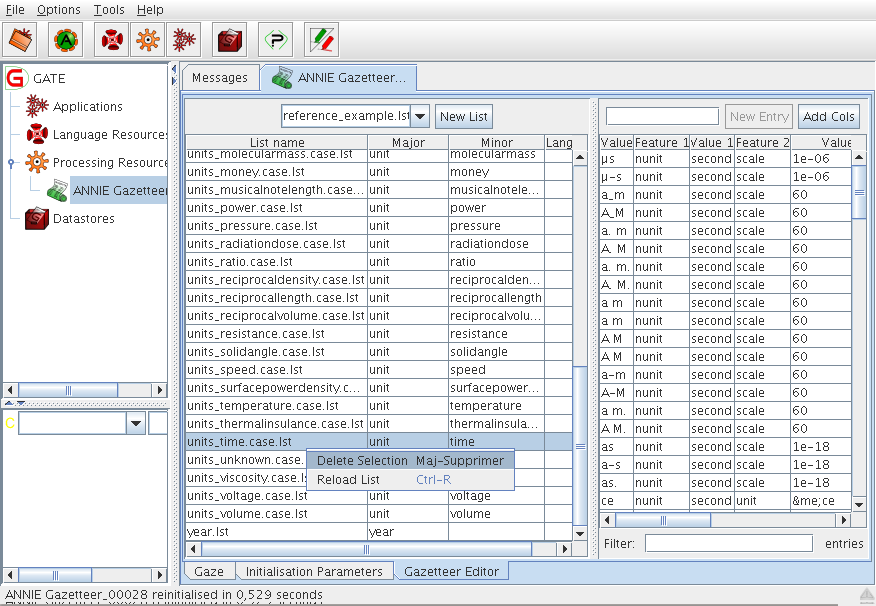
\includegraphics[scale=0.5]{annie-gazetteer-editor.png}
\end{center}
\caption{ANNIE Gazetteer Editor}
\label{fig:anniegazeditor}
\end{figure}

To open this edior, double-click on the
gazetteer in the resources tree.

It is composed of two tables:
\begin{itemize}
\item a left table with 5 columns (List name, Major, Minor, Language, Annotation type) for the
  index, usually a .def file
\item a right table with 1+2*n columns (Value, Feature 1, Value 1...Feature
n, Value n) for the lists, usually .lst files
\end{itemize}

When selecting a list in the left table you get its content displayed in the
right table.

You can sort both tables by clicking on their column headers. A text field
`Filter' at the bottom of the right table allows to display only the rows
that contain the expression you typed.

To edit a value in a table, double click on a cell or press F2 then press
Enter when finished editing the cell. To add a new row in both tables use
the text field at the top and press Enter or use the `New' button next to
it. When adding a new list you can select from the list of existing
gazetteer lists in the current directory or type a new file name. To delete
a row, press Shift+Delete or use the context menu. To delete more than one
row select them before.

You can reload a modified list by selecting it and right-clicking for the
context menu item `Reload List' or by pressing Control+R. When a list is
modified its name in the left table is coloured in red.

If you have set `gazetteerFeatureSeparator' parameter then the right table
will show a `Feature' and `Value' columns for each feature. To add a new
couple of columns use the button `Add Cols'.

Note that in the left table, you can only select one row at a time.

The gazetteer like other language resource has a context menu in the
resources tree to `Reinitialise', `Save' or `Save as...' the resource.

The right table has a context menu for the current selection to help you
creating new gazetteer. It is similar with the actions found in a
spreadsheet application like `Fill Down Selection', `Clear Selection', `Copy
Selection', `Paste Selection', etc.

%%%%%%%%%%%%%%%%%%%%%%%%%%%%%%%%%%%%%%%%%%%%%%%%%%%%%%%%%%%%%%%%%%%%%%%%%%%%%
\sect[sec:gazetteers:ontogaz]{OntoGazetteer}
%%%%%%%%%%%%%%%%%%%%%%%%%%%%%%%%%%%%%%%%%%%%%%%%%%%%%%%%%%%%%%%%%%%%%%%%%%%%%

The Ontogazetteer, or Hierarchical Gazetteer, is a processing resource which
can associate the entities from a specific gazetteer list with a class
in a GATE ontology language resource.  
The OntoGazetteer assigns classes rather than major or
minor types, and is aware of mappings between lists and class
IDs. The Gaze visual resource can display the lists, ontology mappings and 
the class hierarchy of the ontology for a OntoGazetteer processing resource 
and provides ways of editing these components.

%%%%%%%%%%%%%%%%%%%%%%%%%%%%%%%%%%%%%%%%%%%%%%%%%%%%%%%%%%%%%%%%%%%%%%%%%%%%%
\sect[sec:gazetteers:onto_gaze]{Gaze Ontology Gazetteer Editor}
%%%%%%%%%%%%%%%%%%%%%%%%%%%%%%%%%%%%%%%%%%%%%%%%%%%%%%%%%%%%%%%%%%%%%%%%%%%%%

This section describes the Gaze gazetteer editor when it displays
an OntoGazetteer processing resource. The editor consists of two
parts: one for the editing of the lists and the mapping of lists and
one for editing the ontology. These two parts are described in the 
following subsections.

\subsect{The Gaze Gazetteer List and Mapping Editor}

This is a VR for editing the gazetteer lists, and mapping them to
classes in an ontology. It provides load/store/edit for the lists,
load/store/edit for the mapping information, loading of ontologies,
load/store/edit for the linear definition file, and mapping of the lists
file to the major type, minor type and language.

\textbf{Left pane:} A single ontology is visualized in the left pane of the VR. 
The mapping between a list and a class is displayed by showing the
list as a subclass with a different icon.
The mapping is specified by drag and drop from the linear definition
pane (in the middle) and/or by right click menu. 

\textbf{Middle pane:} The middle pane displays the nodes/lines in the
linear definition file. 
By double clicking on a node the corresponding list is opened. 
Editing of the line/node is done by right clicking and choosing
edit: a dialogue appears (lower part of the scheme) allowing the
modification of the members of the node. 

\textbf{Right pane:} In the right pane a single gazetteer list is
displayed. It can be edited and parts of it can be
cut/copied/pasted. 

%%%%%%%%%%%%%%%%%%%%%%%%%%%%%%%%%%%%%%%%%%%%%%%%%%%%%%%%%%%%%%%%%%%%%%%%%%%%%%%%%%
\subsect{The Gaze Ontology Editor}
%%%%%%%%%%%%%%%%%%%%%%%%%%%%%%%%%%%%%%%%%%%%%%%%%%%%%%%%%%%%%%%%%%%%%%%%%%%%%%%%%%

Note: to edit ontologies within gate, the more recent ontology viewer editor
provided by the \texttt{Ontology\_Tools} which provides many more features 
can be used, see section~\ref{sec:ontologies:vr}. 

This is a VR for editing the class hierarchy of an ontology. it
provides storing to and loading from RDF/RDFS, and provides
load/edit/store of the class hierarchy of an ontology.

\textbf{Left pane:}
The various ontologies loaded are listed here. On double click or
right click and edit from the menu the ontology is visualized in the
Right pane. 
	
\textbf{Right pane:} 
Besides the visualization of the class hierarchy of the
ontology the following operations are allowed: 
\begin{itemize}
\item expanding/collapsing parts of the ontology
\item adding a class in the hierarchy: by right clicking on the
intended parent of the new class and choosing add sub class. 
\item removing a class: via right clicking on the class and choosing
remove. 
\end{itemize}

As a result of this VR, the ontology definition file is
affected/altered. 

	
%%%%%%%%%%%%%%%%%%%%%%%%%%%%%%%%%%%%%%%%%%%%%%%%%%%%%%%%%%%%%%%%%%%%%%%%%%%%%%%%%%

%%%%%%%%%%%%%%%%%%%%%%%%%%%%%%%%%%%%%%%%%%%%%%%%%%%%%%%%%%%%%%%%%%%%%%
\sect[sec:gazetteers:hash]{Hash Gazetteer}
%%%%%%%%%%%%%%%%%%%%%%%%%%%%%%%%%%%%%%%%%%%%%%%%%%%%%%%%%%%%%%%%%%%
%% TODO: is this actually the HashGazetteer (this was OntotextGazetteer, 
%% something nowhere to be found in current GATE)
%% The HashGazetteer source code is not in GATE and only a jar
%% ontotext.jar is included
%%
The Hash Gazetteer is a gazetteer implemented by the OntoText Lab
(\url{http://www.ontotext.com/}). Its implementation is based on simple lookup
in several java.util.HashMap objects, and is inspired by the strange idea of
Atanas Kiryakov, that searching in HashMaps may be faster than in a Finite State
Machine (FSM).  The Hash Gazetteer processing resource is part of the ANNIE
plugin.

This gazetteer processing resource is implemented in the following way: Every
phrase {i.e. every list entry} is separated into several parts. The parts are
determined by the whitespaces lying among them; e.g., the phrase ``form is
emptiness'' has three parts: ``form'', ``is'', and ``emptiness''.  There is also
a list of HashMaps: mapsList which has as many elements as the longest (in terms
of `count of parts') phrase in the lists. So the first part of a phrase is
placed in the first map. The first part + space + second part is placed in the
second map, etc. The full phrase is placed in the appropriate map, and a
reference to a Lookup object is attached to it.

On first sight it seems that this algorithm is certainly much more
memory-consuming than a finite state machine (FSM) with the parts of the phrases
as transitions, but this is actually not so important since the average length
of the phrases (in parts) in the lists is 1.1.  On the other hand, one advantage
of the algorithm is that, although unconventional, it takes less memory and may
be slightly faster, especially if you have a very large gazetteer (e.g.,
100,000s of entries).
% on average it takes four
% times less memory and works three times faster than an optimized FSM
% implementation.

\subsect{Prerequisites}

The phrases to be recognised should be listed in a set of files, one for
each type of occurrence (as for the standard gazetteer).

The gazetteer is built with the information from a file that contains the set
of lists (which are files as well) and the associated type for each list.
The file defining the set of lists should have the following syntax: each
list definition should be written on its own line and should contain:
\begin{itemize}
\item the file name (required)
\item the major type (required)
\item the minor type (optional)
\item the language(s) (optional)
\end{itemize}

The elements of each definition are separated by `:'. The following is an
example of a valid definition:
\begin{small}
\begin{verbatim}
personmale.lst:person:male:english
\end{verbatim}
\end{small}
Each file named in the lists definition file is just a list containing
one entry per line.

When this gazetteer is run over some input text (a GATE document) it
will generate annotations of type Lookup having the attributes specified in
the definition file.

\subsect{Parameters}

The Hash Gazetteer processing resource allows the specification of the
following parameters when it is created:
\begin{description}
\item[caseSensitive:] this can be switched between \texttt{true} and 
\texttt{false} to indicate if matches should be done in a case-sensitive 
way.
\item[encoding:] the encoding of the gazetteer lists
\item[listsURL:] the URL of the list definitions (index) file, i.e. the
file that contains the filenames, major types and optionally minor types
and languages of all the list files.
\end{description}

There is one run-time parameter, \textbf{annotationSetName} that allows 
the specification of the annotation set in which the Lookup annotations
will be created. If nothing is specified the default annotation set
will be used.


Note that the Hash Gazetteer does not have the \textbf{longestMatchOnly} and
\textbf{wholeWordsOnly} parameters; if you need to configure these options, you
should use the another gazetteer that supports them, such as the standard ANNIE
Gazetteer (see section~\ref{sec:gazetteers:anniegaz}).
%%%%%%%%%%%%%%%%%%%%%%%%%%%%%%%%%%%%%%%%%%%%%%%%%%%%%%%%%%%%%%%%%%%%%%%%%%%%%
\sect[sec:gazetteers:flexgazetteer]{Flexible Gazetteer}
%%%%%%%%%%%%%%%%%%%%%%%%%%%%%%%%%%%%%%%%%%%%%%%%%%%%%%%%%%%%%%%%%%%%%%%%%%%%%

The Flexible Gazetteer provides users with the flexibility to choose their own
customized input and an external Gazetteer. For example, the user might want to replace
words in the text with their base forms (which is an output of the Morphological
Analyser) before running the Gazetteer.

The Flexible Gazetteer performs lookup over a document based on the
values of an arbitrary feature of an arbitrary annotation type, by using an
\textit{externally provided} gazetteer. It is important to use an external gazetteer as
this allows the use of any type of gazetteer (e.g. an Ontological gazetteer).

Input to the Flexible Gazetteer:

Runtime parameters:

\begin{itemize}

\item Document -- the document to be processed

\item \textbf{inputASName} The annotationSet where the Flexible
Gazetteer should search for the AnnotationType.feature specified in the
inputFeatureNames.

\item \textbf{outputASName} The AnnotationSet where Lookup
annotations should be placed.

Creation time parameters:

\item \textbf{inputFeatureNames} -- when selected, these feature values are used to
replace the corresponding original text.  For each feature, a temporary document is 
created from the values of the specified features on the specified annotation types. For
example: for Token.root the temporary document will have content of every Token 
replaced with its root value.  In case of overlapping annotations of the same type in 
the input, only the value of the first annotation is considered.  Here, please note that 
the order of annotations is decided by using the gate.util.OffsetComparator class.

\item \textbf{gazetteerInst} -- the actual gazetteer instance, which should run
over a temporary document. This generates the Lookup annotations with features.
This must be an instance of {\tt gate.creole.gazetteer.Gazetteer} which has
already been created. All such instances will be shown in the dropdown menu
for this parameter in GATE Developer.

\end{itemize}

Once the external gazetteer has annotated text with Lookup annotations, Lookup
annotations on the temporary document are converted to Lookup annotations on the
original document. Finally the temporary document is deleted.

%%%%%%%%%%%%%%%%%%%%%%%%%%%%%%%%%%%%%%%%%%%%%%%%%%%%%%%%%%%%%%%%%%%%%%%%%%%%%
\sect[sec:gazetteers:listscollector]{Gazetteer List Collector}
%%%%%%%%%%%%%%%%%%%%%%%%%%%%%%%%%%%%%%%%%%%%%%%%%%%%%%%%%%%%%%%%%%%%%%%%%%%%%
The gazetteer list collector, found in the Tools plugin, collects occurrences of
entities directly from a set of annotated training documents and populates
gazetteer lists with the entities. The entity types and structure of the
gazetteer lists are defined as necessary by the user. Once the lists have been
collected, a semantic grammar can be used to find the same entities in new
texts.

The target gazetteer must contain a list corresponding exactly to each
annotation type to be collection (for example, \texttt{Person.lst} for the
\texttt{Person} annotations, \texttt{Organization.lst} for the
\texttt{Organization} annotations, etc.).  You can use the gazetteer editor to
create new empty lists for types that are not already in your gazetteer.  Note
that if you do this, you will need to ``Save and Reinitialise'' the gazetteer
later (the collector updates the \texttt{*.lst} files on disk, but not the
\texttt{lists.def} file).

If a list in the gazetteer already contains entries, the collector will add new
entries, but it will only collect one occurrence of each new entry; it checks
that the entry is not present already before adding it.


There are 4 runtime parameters:
\begin{itemize}
\item annotationTypes: a list of the annotation types that should be collected
\item gazetteer: the gazetteer where the results will be stored (this must be
  already loaded in GATE)
\item markupASname: the annotation set from which the annotation types should be
  collected
\item theLanguage: sets the language feature of the gazetteer lists to be
  created to the appropriate language (in the case where lists are collected for
  different languages)
\end{itemize}

Figure \ref{fig:list_collector_snapshot} shows a screenshot of a set of lists
collected automatically for the Hindi language. It contains 4 lists: Person,
Organisation, Location and a list of stopwords. Each list has a majorType whose
value is the type of list, a minorType `inferred' (since the lists have been
inferred from the text), and the language `Hindi'.
%%
\begin{figure*}[htbp]
\begin{center}
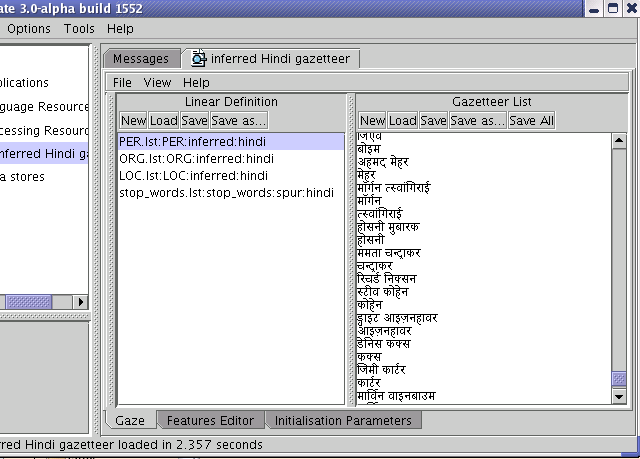
\includegraphics[scale=0.5]{list_collector_snapshot.png}
\end{center}
\caption{Lists collected automatically for Hindi}
\label{fig:list_collector_snapshot}
\end{figure*}


The list collector also has a facility to split the Person names that it
collects into their individual tokens, so that it adds both the entire name to
the list, and adds each of the tokens to the list (i.e. each of the first names,
and the surname) as a separate entry. When the grammar annotates Persons, it can
require them to be at least 2 tokens or 2 consecutive Person Lookups. In this
way, new Person names can be recognised by combining a known first name with a
known surname, even if they were not in the training corpus. Where only a single
token is found that matches, an Unknown entity is generated, which can later be
matched with an existing longer name via the orthomatcher component which
performs orthographic coreference between named entities. This same procedure
can also be used for other entity types. For example, parts of Organisation
names can be combined together in different ways. The facility for splitting
Person names is hardcoded in the file
gate/src/gate/creole/GazetteerListsCollector.java and is commented.
%%
%%%%%%%%%%%%%%%%%%%%%%%%%%%%%%%%%%%%%%%%%%%%%%%%%%%%%%%%%%%%%%%%%%%%%%%%%%%%%
\sect[sec:gazetteers:ontoRootGaz]{OntoRoot Gazetteer}
%%%%%%%%%%%%%%%%%%%%%%%%%%%%%%%%%%%%%%%%%%%%%%%%%%%%%%%%%%%%%%%%%%%%%%%%%%%%%

OntoRoot Gazetteer is a type of a dynamically created gazetteer that
is, in combination with few other generic GATE resources, capable of
producing ontology-based annotations over the given content with
regards to the given ontology. This gazetteer is a part of
`Gazetteer\_Ontology\_Based' plugin that has been developed as a part
of the \htlink{http://www.tao-project.eu}{TAO project}.

%%%%%%%%%%%%%%%%%%%%%%%%%%%%%%%%%%%%%%%%%%%%%%%%%%%%%%%%%%%%%%%%%%%%%%%%%%%%%
\subsect[sec:gazetteers:ontoRootGaz:howDoesItWork]{How Does it Work?}
%%%%%%%%%%%%%%%%%%%%%%%%%%%%%%%%%%%%%%%%%%%%%%%%%%%%%%%%%%%%%%%%%%%%%%%%%%%%%

To produce ontology-based annotations i.e. annotations that link to the specific
concepts or relations from the ontology, it is essential to pre-process the
Ontology Resources (e.g., Classes, Instances, Properties) and extract their
human-understandable lexicalisations.

As a precondition for extracting human-understandable content from the ontology,
first a list of the following is being created:
\begin{itemize}
\item names of all ontology resources i.e. fragment identifiers
\footnote{An ontology resource is usually
identified by an URI concatenated with a set of characters starting with `\#'.
This
set of characters is called \emph{fragment identifier}. For example, if the URI
of a class representing \emph{GATE POS Tagger} is:
'http://gate.ac.uk/ns/gate-ontology\#POSTagger', the fragment identifier will be
'POSTagger'.}
 and
\item assigned property values for all ontology resources (e.g., label and
datatype property values)
\end{itemize}

Each item from the list is further processed so that:
\begin{itemize}
 \item any name containing dash (\verb+"-"+) or underline (\verb+"_"+)
character(s) is processed so
that each of these characters is replaced by a blank space. For example,
 \verb+Project_Name+ or \verb+Project-Name+
would become a \verb+Project Name+.
\item any name that is written in \emph{camelCase} style is actually split
into its constituent words, so that \verb+ProjectName+ becomes  a
\verb+Project Name+ (optional).
\item any name that is a compound name such as `POS Tagger for Spanish' is
split so that both `POS Tagger' and `Tagger' are added to the list for
processing. In this example, `for' is a stop word, and any words after it are
ignored (optional).
\end{itemize}

Each item from this list is analysed separately by the Onto Root Application
(ORA) on execution (see figure~\ref{fig:ontoRootGaz}). The Onto Root Application
first tokenises each linguistic term, then assigns part-of-speech and lemma
information to each token.

%\clearpage
\begin{figure}
\begin{center}
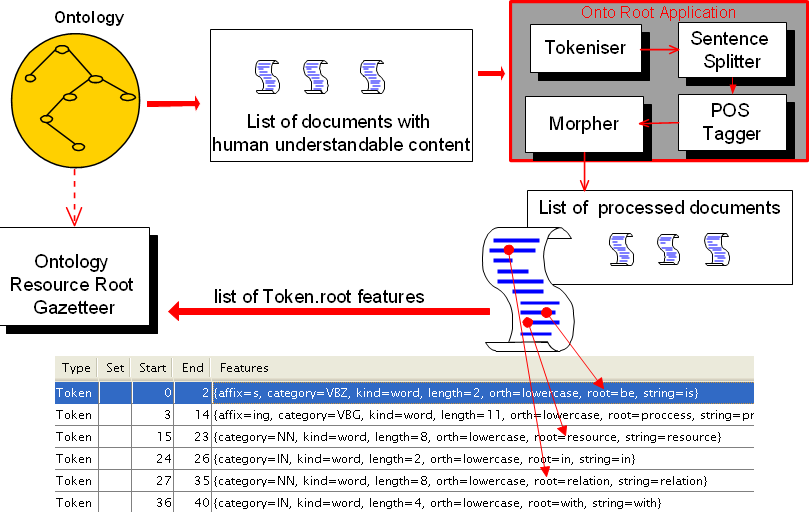
\includegraphics[width=12cm]{ontoRootGaz.png} \ \
\caption{Building Ontology Resource Root (OntoRoot) Gazetteer from the Ontology}
\label{fig:ontoRootGaz}
\end{center}
\end{figure}
As a result of that pre-processing, each token in the terms will have additional
feature named `root', which contains the lemma as created by the morphological
analyser. It is this lemma or a set of lemmas which are then added to the
dynamic gazetteer list, created from the ontology.

For instance, if there is a resource with a short name (i.e., fragment
identifier) \emph{ProjectName}, without any assigned properties the created list
before executing the OntoRoot gazetteer collection  will contain the following
strings:
\begin{itemize}
\item `\emph{ProjectName}',
\item `\emph{Project Name}' after separating camelCased word and
\item `\emph{Name}' after applying heuristic rules.
\end{itemize}

Each of the item from the list is then analysed separately and the results
would be the same as the input strings, as all of entries are nouns given in
singular form.

%%%%%%%%%%%%%%%%%%%%%%%%%%%%%%%%%%%%%%%%%%%%%%%%%%%%%%%%%%%%%%%%%%%%%%%%%%%%%
\subsect[sec:gazetteers:ontoRootGaz:init]{Initialisation of OntoRoot
Gazetteer}
%%%%%%%%%%%%%%%%%%%%%%%%%%%%%%%%%%%%%%%%%%%%%%%%%%%%%%%%%%%%%%%%%%%%%%%%%%%%%

To initialise the gazetteer there are few mandatory parameters:
\begin{itemize}
\item \emph{Ontology} to be processed;
\item \emph{CorpusController} to process the ontology terms\footnote{In
  previous versions of GATE the gazetteer took three separate parameters for
  the tokeniser, POS tagger and morphological analyser.  Existing saved
  applications that use these parameters will still work in GATE 8.0.}.  This
  application will be run on a document that contains a single \verb!Sentence!
  annotation spanning the whole document, and is expected to produce
  annotations of type \verb!Token! in the default annotation set, with features
  \verb!category!  (the POS tag) and \verb!root! (the morphological root).
  Typically this pipeline would contain a tokeniser appropriate to the source
  language, a POS tagger, and a GATE Morphological Analyser PR, but any
  application that will produce the right annotation types and features will
  work.  For example, when processing non-English text you may need to use an
  alternative POS tagger such as the Stanford tagger or TreeTagger.
\end{itemize}

and few optional ones:
\begin{itemize}
\item \emph{useResourceUri}, default is set to true - should this gazetteer
analyse resource URIs or not;
\item \emph{considerProperties}, default is set to true - should this gazetteer
consider properties or not;
\item \emph{propertiesToInclude} - checked only if \emph{considerProperties} is
set to true - this
  parameter contains the list of property names (URIs) to be included, 
  comma separated;
\item \emph{propertiesToExclude} - checked only if \emph{considerProperties} is
set to true -
  this parameter contains the list of property names to be excluded, comma 
  separated;
\item \emph{caseSensitive}, default set to be false -should this gazetteer
differentiate on case;
\item \emph{separateCamelCasedWords}, default set to true - should this
gazetteer separate emph{camelCased} words, e.g. `ProjectName' into `Project
Name';
\item \emph{considerHeuristicRules}, default set to false - should this
gazetteer consider several heuristic rules or not. Rules include splitting the
words containing spaces, and using prepositions as stop words; for example, if
'pos tagger for Spanish' would be analysed, `for' would be considered as a stop
word; heuristically derived would be `pos tagger' and this would be further
used to add `pos tagger' to the gazetteer list, with a feature emph{heuristical
level} set to be 0, and `tagger' with emph{heuristical
level} 1; at runtime lower heuristical level
should be preferred. NOTE: setting \emph{considerHeuristicRules} to true can
cause a lot of noise for some ontologies and is likely to require implementing
an additional filtering resource that will prefer the annotations with the
lower heuristic level;
\end{itemize}


The OntoRoot Gazetteer's initialization preprocesses strings from the ontology
and runs the root finder application over them.  It is possible to re-use the
same tokeniser, POS tagger and morphological analyser PR instances in both the
root finder application and the main pipeline that will contain the finished
OntoRoot Gazetteer, but in this case the PRs \emph{must} use the default
annotation set for output.  If you need to use a different annotation set for
your main pipeline's output then you will need to create separate PRs
specifically for the root finder and configure those to use the default set.
%
%%%%%%%%%%%%%%%%%%%%%%%%%%%%%%%%%%%%%%%%%%%%%%%%%%%%%%%%%%%%%%%%%%%%%%%%%%%%%
\subsect[sec:gazetteers:ontoRootGaz:steps]{Simple steps to run OntoRoot
Gazetteer}
%%%%%%%%%%%%%%%%%%%%%%%%%%%%%%%%%%%%%%%%%%%%%%%%%%%%%%%%%%%%%%%%%%%%%%%%%%%%%

OntoRoot Gazetteer is a part of the Gazetteer\_Ontology\_Based plugin.

%%%%%%%%%%%%%%%%%%%%%%%%%%%%%%%%%%%%%%%%%%%%%%%%%%%%%%%%%%%%%%%%%%%%%%%%%%%%%
\subsubsect[sec:gazetteers:ontoRootGaz:init:easy]{Easy way}
%%%%%%%%%%%%%%%%%%%%%%%%%%%%%%%%%%%%%%%%%%%%%%%%%%%%%%%%%%%%%%%%%%%%%%%%%%%%%
For a quick start with the OntoRoot Gazetteer, consider running it from the
GATE Developer (GATE GUI):
\begin{itemize}
\item Start GATE
\item Load a sample application from resources folder (exampleApp.xgapp). This
will load \emph{CAT App} application.
\item Run \emph{CAT App} application and open \emph{query-doc} to see a
set of Lookup annotations generated as a result (see
Figure~\ref{fig:ontoRoot-sample-annotation}).
\end{itemize}

\begin{figure}
\begin{center}
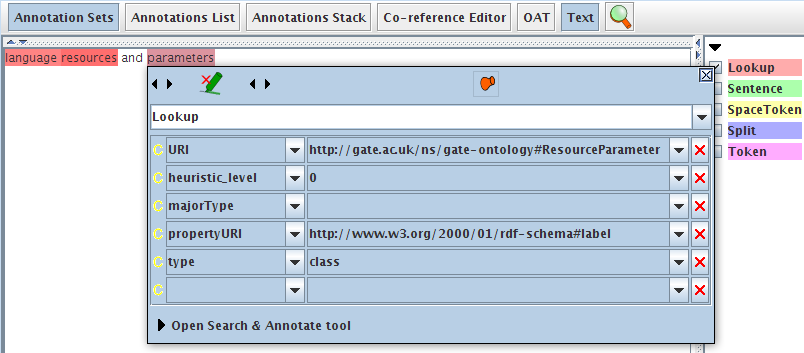
\includegraphics[width=12cm]{ontoRoot-sample-annotation.png} \ \
\caption{Sample ontology-based annotation as a result of running OntoRoot
Gazetteer. Feature \emph{URI} refers to the URI of the ontology resource, while
\emph{type} identifies the type of the resource such as \emph{class, instance,
property}, or \emph{datatypePropertyValue}}
\label{fig:ontoRoot-sample-annotation}
\end{center}
\end{figure}

%%%%%%%%%%%%%%%%%%%%%%%%%%%%%%%%%%%%%%%%%%%%%%%%%%%%%%%%%%%%%%%%%%%%%%%%%%%%%
\subsubsect[sec:gazetteers:ontoRootGaz:init:hard]{Hard way}
%%%%%%%%%%%%%%%%%%%%%%%%%%%%%%%%%%%%%%%%%%%%%%%%%%%%%%%%%%%%%%%%%%%%%%%%%%%%%.

OntoRoot Gazetteer can easily be set up to be used with any ontology. To
generate a GATE application which demonstrates the use of the OntoRoot
Gazetteer, follow these steps:
\begin{enumerate}
 \item Start GATE
 \item Load necessary plugins: Click on \emph{Manage CREOLE plugins} and check
the following:
      \begin{itemize}
       \item Tools
       \item Ontology
       \item Ontology\_Based\_Gazetteer
       \item Ontology\_Tools (optional); this parameter is required in order to
view ontology using the GATE Ontology Editor.
       \item ANNIE.
      \end{itemize}
Make sure that these plugins are loaded from GATE/plugins/[plugin\_name] folder.
  \item Load an ontology. Right click on \emph{Language Resource}, and select
the last option to create an \emph{OWLIM Ontology LR}. Specify the format 
of the ontology, for example \emph{rdfXmlURL}, and give the correct path to the 
ontology: either the absolute path on your local machine such as 
\texttt{c:/myOntology.owl} or the URL such as
\texttt{http://gate.ac.uk/ns/gate-ontology}.
Specify the \emph{name} such as \emph{myOntology} (this is
optional).
  \item Create Processing Resources: Right click on the \emph{Processing
Resource} and create the following PRs (with default parameters):
\begin{itemize}
 \item Document Reset PR
 \item ANNIE English Tokeniser
 \item ANNIE POS Tagger
 \item GATE Morphological Analyser
 \item RegEx Sentence Splitter (or ANNIE Sentence Splitter)
\end{itemize}

Place the tokeniser, POS tagger and morphological analyser PRs into a new
``corpus pipeline'' application, named ``Root finder''.

\item Create an \emph{Onto Root Gazetteer} and set the init parameters.
Mandatory ones are:
\begin{itemize}
 \item \emph{ontology}: select previously created myOntology;
 \item \emph{rootFinderApplication}: select the ``Root finder'' pipeline you
   created above.
\end{itemize}
OntoRoot gazetteer is quite flexible in that it can be configured using the
optional parameters. List of all parameters is detailed in
Section~\ref{sec:gazetteers:ontoRootGaz:init}.

When all parameters are set click OK. It can take some time to
initialise OntoRoot Gazetteer. For example, loading GATE knowledge base from
 \texttt{http://gate.ac.uk/ns/gate-kb} takes around 6-15 seconds. Larger
ontologies can take much longer.
 \item Create another PR which is a Flexible Gazetteer. As init parameters
it is
 mandatory to select previously created OntoRoot Gazetteer for gazetteerInst.
 For another parameter, inputFeatureNames, click on the button on the right
 and when prompt with a window, add 'Token.root' in the provided textbox, then
 click Add button. Click OK, give name to the new PR (optional) and then click 
 OK.
\item Create an application. Right click on Application, then create a new
Corpus Pipeline (or Conditional Corpus Pipeline). Add the following PRs to the
application in this particular order:
\begin{itemize}
 \item Document Reset PR
 \item RegEx Sentence Splitter (or ANNIE Sentence Splitter)
 \item ANNIE English Tokeniser
 \item ANNIE POS Tagger
 \item GATE Morphological Analyser
 \item Flexible Gazetteer
\end{itemize}

The tokeniser, POS tagger and morphological analyser may be the same ones used
in the root finder application, or they may be different (and must be different
if you want to use an annotation set other than the default one for this
pipeline's PRs).

\item Create a document to process with the new
application; for example, if the ontology was
\texttt{http://gate.ac.uk/ns/gate-kb}, then the document could be the GATE home
page: \texttt{http://gate.ac.uk}. Run application and then investigate the
results further.
All annotations are of type \emph{Lookup}, with additional features that give
details
about the resources they are referring to in the given ontology.
\end{enumerate}

%%%%%%%%%%%%%%%%%%%%%%%%%%%%%%%%%%%%%%%%%%%%%%%%%%%%%%%%%%%%%%%%%%%%%%%%%%%%%
\sect[sec:gazetteers:lkb-gazetteer]{Large KB Gazetteer}
%%%%%%%%%%%%%%%%%%%%%%%%%%%%%%%%%%%%%%%%%%%%%%%%%%%%%%%%%%%%%%%%%%%%%%%%%%%%%

\textit{Note that from GATE 8.5 onwards the ontology plugin must have been
loaded before you can load this plugin. The plugin also does not appear in
the default list. It can be added by providing it's Maven coordinates through
the plugin manager. See \url{https://github.com/GateNLP/gateplugin-Gazetteer_LKB}
for more information about the plugin and how to load it.}

The large KB gazetteer provides support for ontology-aware NLP. You can load
any ontology from RDF and then use the gazetteer to obtain lookup annotations
that have both instance and class URI. Alternately, the PR can read in
LST and DEF files in the same format as the Default Gazetteer. For both
data sources, the Large KB Gazetteer PR allows to use large gazetteer
lists and speeds up subsequent loading of the data by caching.

The large KB gazetteer is available as the plugin \texttt{Gazetteer\_LKB}.

The current version of the large KB gazetteer does not use GATE ontology
language resources. Instead, it uses its own mechanism to load and
process ontologies. 

The Large KB gazetteer grew from a component in the semantic search platform
\htlink{http://ontotext.com/kim/}{Ontotext KIM}. The gazetteer was developed by
people from the KIM team. You
may find the name \pitalic{kim} left in several places in the source code,
documentation or source files.

\subsect{Quick usage overview}

\begin{itemize}
\item{} To use the Large KB gazetteer, set up your dictionary first. The
dictionary is a folder with some configuration files. Use the samples at
\pitalic{GATE\_HOME/plugins/Gazetteer\_LKB/samples} as a guide. There are 
samples for loading the gazetteer data from a local repository, a remote
repository or from a set of list files as configured in a \texttt{.def} file.

\item{} Load \pitalic{GATE\_HOME/plugins/Gazetteer\_LKB} as a CREOLE plugin.
See Section~\ref{sec:developer:plugins} for details.

\item{} Create a new `Large KB Gazetteer' processing resource (PR). Put the
folder of the dictionary you created in the `dictionaryPath' parameter. You can
leave the rest of the parameters as defaults.

\item{} Add the PR to your GATE application. The gazetteer doesn't require a
tokenizer or the output of any other processing resources.

\item{} The gazetteer will create annotations with type `Lookup' and two
features; `inst', which contains the URI of the ontology instance, and `class'
which contains the URI of the ontology class that instance belongs to. If
the gazetteer was loaded from gazetteer list files, the `inst' and `class'
features are set from the `minorType' and `majorType' settings for the list
file or from the `inst' and `class' features stored for each entry in
the list file (see below).
\end{itemize}

\subsect{Dictionary setup}

The dictionary is a folder with some configuration files. You can find samples at
\pitalic{GATE\_HOME/plugins/Gazetteer\_LKB/samples}.

Setting up your own dictionary is easy. You need to define your RDF ontology
and then specify a SPARQL or SERQL query that will retrieve a subset of that
ontology as a dictionary.

\pitalic{config.ttl} is a Turtle RDF file which configures a local RDF
ontology or connection to a remote Sesame RDF database.

If you want to see examples of how to use local RDF files, please check
\pitalic{samples/dictionary\_from\_local\_ontology/config.ttl}. The
\pitalic{Sesame repository configuration} section configures a local
\htlink{http://ontotext.com/owlim/}{Ontotext SwiftOWLIM} database that loads a
list of RDF files. Simply create a list of your RDF files and reuse the rest of
the configuration. The sample configuration support datasets with 10,000,000
triples with acceptable performance. For working with larger datasets, advanced
users can substitute SwiftOWLIM with another Sesame RDF engine. In that case,
make sure you add the necessary JARs to the list in
\pitalic{GATE\_HOME/plugins/Gazetteer\_LKB/creole.xml}. For example,
\htlink{http://www.ontotext.com/owlim/big/}{Ontotext BigOWL} is a Sesame RDF
engine that can load billions of triples on desktop hardware.

Since any Sesame repository can be configured in \pitalic{config.ttl}, the Large
KB Gazetteer can extract dictionaries from \pbold{all} significant RDF databases.
See the page on
\htlink{http://nmwiki.ontotext.com/lkb\string_gazetteer/database\string_compatibility.html}{database compatibility} for more information.

\pitalic{query.txt} contains a SPARQL query. You can write any query you like,
as long as its projection contains at least two columns in the following
order: label and instance. As an option, you can also add a third column for
the ontology class of the RDF entity. Below you can see a sample query, which
creates a dictionary from the names and the unique identifiers of 10,000
entertainers in DbPedia.

\begin{pverbatimbox}
\begin{small}\begin{verbatim}
PREFIX opencyc: <http://sw.opencyc.org/2008/06/10/concept/en/>
PREFIX rdfs: <http://www.w3.org/2000/01/rdf-schema#>

SELECT ?Name ?Person WHERE {
        ?Person a opencyc:Entertainer ; rdfs:label ?Name .           
    FILTER (lang(?Name) = "en") 
} LIMIT 10000
\end{verbatim}\end{small}
\end{pverbatimbox}

Try this query at the \htlink{http://ldsr.ontotext.com/}{Linked Data Semantic
Repository}.

When you load the dictionary configuration in GATE for the first time, it
creates a binary snapshot of the dictionary. Thereafter it will load only this
binary snapshot. If the dictionary configuration is changed, the snapshot will
be reinitialized automatically. For more information, please see the
\htlink{http://nmwiki.ontotext.com/lkb\string_gazetteer/dictionary\string_lifecycle.html}{dictionary
lifecycle specification}.

\subsect{Additional dictionary configuration}

The config.ttl may contain additional dictionary configuration. Such
configuration concerns only the initial loading of the dictionary from the RDF
database. The options are still being determined and more will appear in
future versions. They must be placed below the repository configuration
section as attributes of a dictionary configuration. Here is a sample
\pitalic{config.ttl} file with additional configuration.

\begin{pverbatimbox}
\begin{small}\begin{verbatim}
# Sesame configuration template for a (proxy for a) remote repository
#
@prefix rdfs: <http://www.w3.org/2000/01/rdf-schema#>.
@prefix rep: <http://www.openrdf.org/config/repository#>.
@prefix hr: <http://www.openrdf.org/config/repository/http#>.
@prefix lkbg: <http://www.ontotext.com/lkb_gazetteer#>.

[] a rep:Repository ;
   rep:repositoryImpl [
      rep:repositoryType "openrdf:HTTPRepository" ;
      hr:repositoryURL <http://ldsr.ontotext.com/openrdf-sesame/repositories/owlim>
   ];
   rep:repositoryID "owlim" ;
   rdfs:label "LDSR" .
   
[] a lkbg:DictionaryConfiguration ; 
  lkbg:caseSensitivity "CASE_INSENSITIVE" .  
\end{verbatim}\end{small}
\end{pverbatimbox}

\subsect{Dictionary for Gazetteer List Files}

In order to load the gazetteer from gazetteer list files,
place a file with extension \texttt{.def} in the dictionary
directory. This file should have the same format as for
the Default Gazetteer, however the fields for language and
annotation type are ignored. The values for the fields
`majorType' and `minorType' are converted to URIs by 
prepending `urn:' and the URI from `majorType' is used for
assigning the `class' feature, the URI from `minorType'
for assigning the `inst' feature of all annotations created
from the list. These valus can be overwritted by features
from the individual entries in a list file, if the
`gazetteerFeatureSeparator' configuaration option is set
to a non-blank value in the configuration file. In that
case, each line in a list file is split by the separator
and the first part is used as the gazetteer entry. The 
remaining parts are interpreted as feature/value pairs
of the form \texttt{feature=value}. If a feature `inst'
is found the value is used as the inst URI for that entry,
overwriting the URI taken from the `minorType' of the list
file. If a feature `class' is found, the value is used as
the class URI for that entry, overwriting the URI taken from
the `majorType' of the list file.

The \texttt{config.ttl} file for a loading the gazetteer
from list files should have the following content (the example
shows a tab character to be used as the feature separator
for list files):

\begin{pverbatimbox}
\begin{small}\begin{verbatim}
@prefix lkbg: <http://www.ontotext.com/lkb_gazetteer#>.
lkbg:DictionaryConfiguration 
   lkbg:caseSensitivity "caseinsensitive" ;
   lkbg:caching "enabled" ;
   lkbg:ignoreList "ignoreList.txt" ;
   lkbg:gazetteerFeatureSeparator "\t" .
\end{verbatim}\end{small}
\end{pverbatimbox}



\subsect{Processing Resource Configuration}

The following options can be set when the gazetteer PR is initialized:

\begin{plist}

\item{} dictionaryPath; the dictionary folder described above.

\item{} forceCaseSensitive; whether the gazetteer should return
case\symbol{45}sensitive matches regardless of the loaded dictionary.

\end{plist}
\subsect{Runtime configuration}

\begin{plist}

\item{} annotationSetName \symbol{45} The annotation set, which will receive
the generated lookup annotations.

\item{} annotationLimit \symbol{45} The maximum number of the generated
annotations. NULL or 0 for no limit. Setting limit of the number of the
created annotations will reduce the memory consumption of GATE on large
documents. Note that GATE documents consume gigabytes of memory if there are
tens of thousands of annotations in the document. All PRs that create large
number of annotations like the gazetteers and tokenizers may cause an Out Of
Memory error on large texts. Setting that option limits the amount of memory
that the gazetteer will use.

\end{plist}

\subsect[sec:gazetteers:semantic-enrichment]{Semantic Enrichment PR}

The Semantic Enrichment PR allows adding new data to semantic annotations by
querying external RDF (Linked Data) repositories. It is a companion to the
large KB gazetteer that showcases the usefulness of using Linked Data URI as
identifiers.

Here a semantic annotation is an annotation that is linked to an RDF entity by
having the URI of the entity in the `inst' feature of the annotation. For all
such annotation of a given type, this PR runs a SPARQL query against the
defined repository and puts a comma\symbol{45}separated list of the values
mentioned in the query output in the `connections' feature of the same
annotation.

There is a \htlink{http://nmwiki.ontotext.com/lkb\string_gazetteer/samples.html}{sample
pipeline} that features the Semantic Enrichment PR.

\subsubsect{Parameters}

\begin{plist}

\item{} inputASName; the annotation set, which annotation will be
processed.

\item{} server; the URL of the Sesame 2 HTTP repository. Support
for generic SPARQL endpoints can be implemented if required.

\item{} repositoryId; the ID of the Sesame repository.

\item{} annotationTypes; a list of types of annotation that will be
processed.

\item{} query; a SPARQL query pattern. The query will be processed
like this \symbol{45} String.format(query, uriFromAnnotation), so you can use
parameters like \%s or \%1\$s.

\item{} deleteOnNoRelations; whether we want to delete the
annotation that weren't enriched. Helps to clean up the input annotations.

\end{plist}



%%%%%%%%%%%%%%%%%%%%%%%%%%%%%%%%%%%%%%%%%%%%%%%%%%%%%%%%%%%%%%%%%%%%%%%%%%%%%
\sect[sec:gazetteers:shared]{The Shared Gazetteer for multithreaded processing}
%%%%%%%%%%%%%%%%%%%%%%%%%%%%%%%%%%%%%%%%%%%%%%%%%%%%%%%%%%%%%%%%%%%%%%%%%%%%%

The \texttt{DefaultGazetteer} (and its subclasses such as the
\texttt{OntoRootGazetteer}) compiles its gazetteer data into a finite state
matcher at initialization time.  For large gazetteers this FSM requires a
considerable amount of memory.  However, once the FSM has been built then (as
long as you do not modify it dynamically using Gaze) it is accessed in a
read-only manner at runtime.  For a multi-threaded application that requires
several identical copies of its processing resources (see
section~\ref{sec:api:multithread}), GATE provides a mechanism whereby a
single compiled FSM can be shared between several gazetteer PRs that can then
be executed concurrently in different threads, saving the memory that would
otherwise be required to load the lists several times.

This feature is not available in the GATE Developer GUI, as it is only intended
for use in embedded code.  To make use of it, first create a single instance
of the regular \texttt{DefaultGazetteer} or \texttt{OntoRootGazetteer}:
%
\begin{small}\begin{verbatim}
FeatureMap params = Factory.newFeatureMap();
params.put("listsUrl", listsDefLocation);
LanguageAnalyser mainGazetteer = (LanguageAnalyser)Factory.createResource(
    "gate.creole.gazetteer.DefaultGazetteer", params);
\end{verbatim}\end{small}

Then create any number of \texttt{SharedDefaultGazetteer} instances, passing
this regular gazetteer as a parameter:
%
\begin{small}\begin{verbatim}
FeatureMap params = Factory.newFeatureMap();
params.put("bootstrapGazetteer", mainGazetteer);
LanguageAnalyser sharedGazetteer = (LanguageAnalyser)Factory.createResource(
    "gate.creole.gazetteer.SharedDefaultGazetteer", params);
\end{verbatim}\end{small}

The \texttt{SharedDefaultGazetteer} instance will re-use the FSM that was built
by the \texttt{mainGazetteer} instead of loading its own.
